%%=========================================
\section[Diskusjon \& Konklusjon]{Diskusjon \& Konklusjon}
%%=========================================
\subsection{Diskusjon}
\subsubsection*{Gestegjenkjennelse gjennom fotodioder}
Eksperimentet oppsummert:
\begin{itemize}
\item Jeg argumenterte for at en gestesensor i form av enkle fotodioder er et tilstrekkelig medium for enkel brukerinteraksjon.
\item Jeg viste at maskinlæring kan benyttes for å lære et system å forstå enkle gester og viste at dette er et alternativ til å eksplisitt programmere forståelse.
\item Jeg viste at det holder med et titalls treningseksempler fra hver gest for å oppnå gode resultater med lineære modeller, og at det med 50 eksempler oppnås en suksessrate på 96\%.
\end{itemize}
\begin{figure}[h!]
\centering
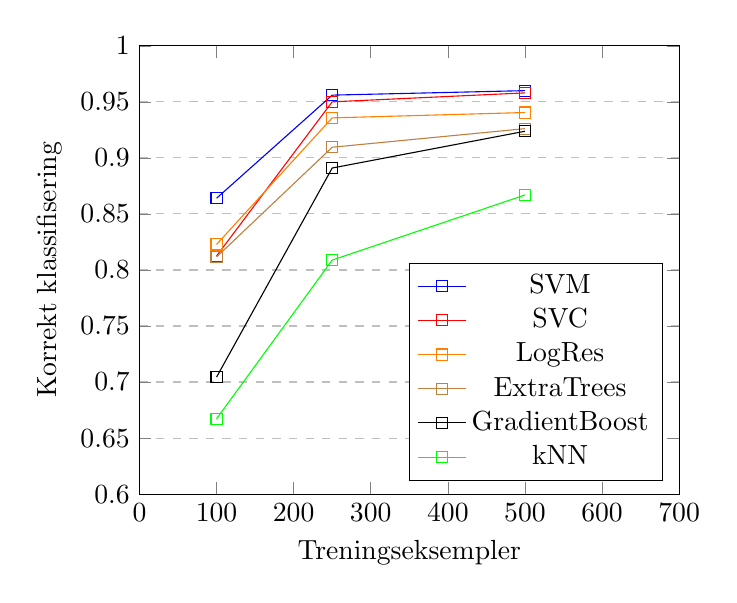
\begin{tikzpicture}
\begin{axis}[
    xlabel={Treningseksempler},
    ylabel={Korrekt klassifisering},
    xmin=0, xmax=700,
    ymin=0.6, ymax=1.0,
    xtick={0,100,200,300,400,500,600,700},
    ytick={0.6,0.65,0.7,0.75,0.8,0.85,0.9,0.95,1.0},
    legend pos=south east,
    ymajorgrids=true,
    grid style=dashed,
]
\addplot[
    color=blue,
    mark=square,
    ]
    coordinates {
    (100,0.864)(250,0.956)(500,0.96)
    };
\addplot[
    color=red,
    mark=square,
    ]
    coordinates {
    (100,0.8124)(250,0.95)(500,0.958)
    };
\addplot[
    color=orange,
    mark=square,
    ]
    coordinates {
    (100,0.8228)(250,0.9357)(500,0.94048)
    };
\addplot[
    color=brown,
    mark=square,
    ]
    coordinates {
    (100,0.8116)(250,0.9095)(500,0.92608)
    };
\addplot[
    color=black,
    mark=square,
    ]
    coordinates {
    (100,0.7044)(250,0.89095)(500,0.92376)
    };
\addplot[
    color=green,
    mark=square,
    ]
    coordinates {
    (100,0.6672)(250,0.8088)(500,0.86688)
    };
    
    \legend{SVM,SVC,LogRes,ExtraTrees,GradientBoost,kNN}
\end{axis}
\end{tikzpicture}
\caption{Resultatsutvikling for et utvalg algoritmer}
\label{fig:resultsgraf}
\end{figure}
Både logistisk regresjon og støttevektormaskin ga svært lovende resultater, som vist i tabell \ref{table:results}. 96\% er en meget høy suksessrate og viser hvor godt enkle, lineære modeller kan skille på denne typen data. Det ble interessant å deretter spørre om dette resultatet kunne blitt enda høyere. Jeg ønsket ikke å bruke mer tid på å lage flere treningseksempler, så i stedet utførte jeg treningen på nytt med færre treningseksempler, i håp om å kunne se en utviklingstrend. Det samme eksperimentet ble utført med en femtedel og halvparten av dataene for å danne et bilde av sammenhengen mellom forbedring i suksessrate og antall treningseksempler. Figur \ref{fig:resultsgraf} viser resultatene for 100, 250 og 500 treningseksempler. Ettersom biblioteket jeg benyttet for å implementere algoritmene tilbyr en rekke andre algoritmer forsøkte jeg noen andre tilnærminger enn lineære modeller og inkluderte dem også.

I figur \ref{fig:resultsgraf} kan vi se at SVM-ene er i nærheten av 95\% allerede etter 250 treningseksempler og at de kun øker minimalt med 250 ekstra tilfeller. Dette tyder på at det trengs et stort antall ekstra treningseksempler for at algoritmene skal krype betydelig nærmere 100\%. De mer kompliserte algoritmene \emph{ExtraTrees} og \emph{GradientBoost} benytter seg av flere algoritmer under panelet og kombinerer disse. Det kan se ut som om spesielt GradientBoost kan fortsette å øke suksessraten betydelig med mer trening, men det er tvilsomt om den noen gang passerer SVM. Til sist nevnes k-nærmeste nabo (kNN), som begynner svakest av de utprøvde algoritmene, men fremdeles har en sterk vekst mellom 250 og 500 tilfeller. Det hadde vært interessant å se utviklingen videre for denne enkle algoritmen.

Dette prosjektet har argumentert for at gester kan være en aktuell interaksjonsform i hjemmet, spesielt som en erstatning til store knappepaneler og desentralisert styringskontroll. Det har også vist at maskinlæring kan benyttes for å gi enkle sensorer en svært god forståelse av gester. Det er dermed vist at det ikke er nødvendig med kameraer for å benytte gester. Med en suksessrate på over 96\% i klassifiseringen av 10 ulike gester er denne teknikken svært interessant. Og med en suksessrate på over 85\% allerede etter kun 10 treningseksempler på hver gest, kan man forestille seg at brukere selv kan sette av 10 minutter til å trene et helt nytt og utrent system til å forstå sine egne gester. I et produkt kunne det vært aktuelt å tilby online-læring gjennom systemets levetid. Man kan med andre ord la systemet lære etter hvert som brukeren benytter systemet. Dette vil nødvendigvis kreve at brukeren har en mulighet til å gi tilbakemelding på når systemet gjettet riktig gest og når det gjettet feil. Jeg har vist at en enkel sensor, gjennom maskinlæring, kan benyttes praktisk som en multifunksjonell bryter med flere tilstander enn hva man kan programmere for hånd.\\

\subsubsection*{Multimodal interaksjon gjennom tale og gester}
Eksperimentet oppsummert:
\begin{itemize}
\item Jeg argumenterte for at tale og gester fungerer best som kommunikasjonsprogramvare.
\item Jeg argumenterte for at kombinasjonen av enkle gester og talekommandoer er en effektiv måte å interagere med det smarte hjemmet på.
\item Jeg viste at talegjenkjenning over en begrenset mengde ord dekker funksjonaliteten vi ønsker å tilby gjennom tale, uten problemer med personvern.
\item Jeg implementerte et system som håndterer multimodal inputdata fra gestesensor og mikrofon. Denne ble benyttet for å simulerer bruken i et smart hjem ved å vise en dynamisk grafisk representasjon av inputdataene.
\end{itemize}
Hypotesen kan sies å være godt utfordret dersom den multimodale interaksjonen kan vises å være tilstrekkelig til å styre hjemmet, at den er naturlig og at den er effektiv. Disse er vanskelige å måle empirisk. Eksperimentet har argumentert for at den begrensede talegjenkjenningen ikke bare er tilstrekkelig, men er en bedre tilnærming enn kontinuerlig tale, med dagens begrensninger i teknologi. Med definisjonene for naturlig og effektiv jeg ga i kapittel 1 trengs det eksperimenter med brukere for å besvare hypotesen. For å avgjøre om interaksjonen er instinktiv, forståelig, enkel i bruk, praktisk og hensiktsmessig må et bredt utvalg brukere observeres mens de tar i bruk systemet. Jeg definerte også ordene slik at naturlig interaksjon må gi rimelige resultater og effektiv interaksjon må gi resultater raskt. I kontekst av det smarte hjemmet kan disse kravene være vanskelig å oppfylle. Dersom du sier til hjemmet at lyset skal skrus av i rommet brukeren befinner seg i, kan resultatet evalueres umiddelbart. Men dersom brukeren bruker systemet for å låse ytterdøra, senke temperaturen eller slå av lyset i et annet rom er det en utfordring å for dette systemet å gi feedback raskt, og å gi feedback som forteller brukeren om resultatet var rimelig.\\

\subsubsection*{Kombinasjoner}
Eksperimentet oppsummert:
\begin{itemize}
\item Jeg argumenterte for at et stort vokabular av abstrakte gester i praksis er et tegnspråk og at retningslinjer som gjelder for taledrevne systemer også gjelder for slike gestedrevne systemer.
\item Jeg viste at de 10 gestene fra eksperiment 1 danner langt bedre data med fire sensorer, og at maskinlæring er enda mer effektivt.
\item Jeg viste at systemet kan trenes til å skille mellom 42 ulike gester med 93\% suksessrate, med kun 10 treningseksempler av hver gest.
\item Jeg argumenterte for at sensorenes nærhetsdeteksjon kan brukes i forbindelse med smarte hjem, for eksempel for å dimme lys og regulere lydvolum.
\end{itemize}
Resultatet fra maskinlæringen bekrefter hypotesen. Om de 42 gestene er naturlige er uvisst og krever brukertesting. Gestene er enkle og bør derfor også være forståelige. Om gestene gir rimelige resultater avhenger av hvordan de anvedes. Jeg vil si at en sveipende gest er like naturlig for å skru av/på et lys, som en tradisjonell knapp er. Det samme gjelder for å regulere nivåer med avstand, mot å skru på et hjul. Andre gester kan kanskje anses som mer abstrakte og mindre naturlige.

I eksperiment 1 økte resultatene fra 86\%, 82\% og 81\% med 10 treningseksempler av hver gest, til 96\%, 96\% og 95\% med 50 treningseksempler av hver gest. Dette er en økning på 11.6\%, 17.1\% og 17.3\%. Dersom vi kan anta en liknende forbedring i 50 treningseksempler av hver av de 42 gestene kan vi forvente resultater som kryper svært nære 100\%.\\

\subsubsection*{Kontekstdrevet brukergrensesnitt}
Eksperimentet oppsummert:
\begin{itemize}
\item Jeg argumenterte for at et grafisk brukergrensesnitt for smarte hjem er informasjonsprogramvare. Brukerene er hovedsaklig interessert i å lære om hjemmet. Informasjonen bør derfor presenteres på en optimal måte, for å oppnå dette målet.
\item Jeg implementerte et brukergrensesnitt som viser hjemmets tilstand og dynamisk tilpasser seg ny informasjon. Grensesnittets utseende forandret seg basert på regler og prioriteringer.
\end{itemize}
Brukergrensesnittet jeg har utviklet og argumentert for forsøker å maksimere utnyttelsen av de rike kontekstdataene et smart hjem tilbyr. Ved å forstå konteksten rundt dataene gjennom regler, kan programvaren hjelpe brukeren med å finne, og lære av, informasjonen som er av interesse. Disse egenskapene gjør brukergrensesnittet til et intelligent brukergrensesnitt.\\

\subsection{Videre arbeid}
\label{ch:videre}
\subsubsection*{Gestegjenkjennelse gjennom fotodioder}
Tre viktige valg ble tatt i dette eksperimentet: hvilke klassifiseringslagoritmer som ble utforsket, antallet treningseksempler og antallet datapunkter i treningseksemplene. Alle disse dimensjonene ville vært interessante å utforske med andre valg. Vil andre algoritmer fungere bedre dersom antallet treningseksempler øker? Teknikker som dyp læring med nevrale nett kan tilnærme mer avanserte funksjoner med tilstrekkelig trening. Kunne resultatene vært bedre med større datavektorer? Med gestene som skaper mange datapunkter blir datapunktene omgjort til gjennomsnittsresultater og vi mister en del presisjon. Treningseksempler med mer data vil kreve flere ressurser fra systemet.

Til sist vil jeg nevne online læring. Man kan utforske et system som lærer etter hvert som brukeren benytter systemet. For at systemet skal lære, er brukeren nødt til å kunne gi beskjed om systemet gjettet riktig eller ikke. Dette kan utforskes med talegjenkjenning og syntesert tale. Et annet alternativ er en liten touchskjerm der brukeren kan svare på om gesten ble gjettet riktig.\\

\subsubsection*{Multimodal interaksjon gjennom tale og gester}
Det umiddelbare videre arbeid for den begrensede talegjenkjenningen virker ganske klart: å implementere \emph{rejecting out of grammar utterances}. Slik systemet står nå vil enhver lyd gjenkjennes som et av ordene eller uttrykkene i vokabularet. Når usikkerheten om en lyd er stor bør en null-verdi gjettes. Dermed unngår man at kremt, host, bakgrunnsstøy og pauselyder blir feilaktig gjenkjent som talekommandoer. Dette er foreløpig ikke implementert i Pocketsphinx.

Et spennende prosjekt ville vært å kombinere begrenset tale for å gi hjemmet kommandoer og kontinuerlig, naturlig tale for å spørre orakelspørsmål (som "hva er værmeldingen for neste fredag?" eller "finn en oppskrift på tacokrydder."). En idé er å la ulike gester aktivere den passende talegjenkjenningen. Ved å utføre den riktige gesten vil systemet, i stedet for den lokale talegjenkjenningen, åpne opp en kobling til en tjeneste, som Google, og lytte etter input. Enkle kommandoer for å styre hjemmet. Naturlig tale for å spørre orakel-spørsmål.

Brukertesting vil være et viktig steg videre for å bevise denne hypotesen. Vil brukere finne det naturlig å prate for å skru av og på apparatene i hjemmet? Er det fordelaktig å ha et sentralt, eller et fåtall sentrale steder å utøve styring fra?\\

\subsubsection*{Kombinasjoner}
Når vi nå har etablert at disse sensorene kan oppnå en forståelse for gester ved hjelp av maskinlæring, dukker det opp andre bruksområder. Spesielt scenarier der det er fordelaktig å unngå fysisk kontakt er interessante. Et eksempel er toaletter og vasker, der en enkel gest kan skylle ned eller starte vannet, og andre gester kan justere vanntemperaturen. Et annet sted der hygiene er svært viktig er på sykehus. Helsepersonell kan styre ulik funksjonalitet på et sykehus, uten å komme i kontakt med knapper, skjermer og dører. Her er det store muligheter for utforskning.

Dersom man benytter systemet slik at det må både tale og gester til for å aktivere funksjonalitet, har man i praksis en 2-veis autentisering. Dette kan dermed brukes som en sikkerhetsmekanisme. En passordfrase av vilkårlig lengde sammen med en eller flere korrekte gester, kan åpne en lås eller gi tilgang til å styre funksjonaliteten i hjemmet. Dette vil være en svært trygg autentisering. Samtidig er den effektiv å utføre og tar minimalt med plass.

Et annet aktuelt applikasjonsområde å utforske er tablets. Hva kunne man fått til dersom slike sensorer ble plassert i hjørnene, på kantene eller på baksiden av en tablet? Gester kunne brukes for å utføre vanlige funksjoner som å scrolle og å navigere mellom app-er eller nettleserfaner. Kanskje helt nye interaksjonsformer nå kunne blitt utforsket. Kunne man utnyttet abstrakte gester i luftrommet rundt tablet-en for å skape god interaksjon?

Mange manipulasjonsprogrammer i dag har store menyer med verktøy og innstillinger man skal velge i. Kunne man benyttet mer av skjermarealet til det primære utviklingsområdet ved å tilby valg av verktøy og innstillinger gjennom tale og gester?\\

\subsubsection*{Kontekstdrevet brukergrensesnitt}
For å gi brukergrensesnittet en grad av intelligens ble det implementert et utvalg regler. Disse definerte hvilken informasjon som var av prioritet og som skulle presenteres for brukeren. En videre utvikling kunne være å la brukere legge inn egne regler, og selv definere hva som er av prioritet. Videre kunne teknikker fra maskinlæring også her benyttes for å la programmet selv lære hva brukeren foretrekker. 

Å knytte brukergrensesnittet til reell sensordata ville vært et viktig steg videre. Man kunne så utforsket hvordan brukere benyttet systemet til å få svar på det de leter etter. Brukertesting av både tradisjonelle interaksjonsdrevne grensesnitt og kontekstdrevne grensesnitt, vil skape empiriske data slik at sammenlikninger og konklusjoner kan trekkes.\\

\subsection{Konklusjon}
Denne oppgaven har tatt for seg et utvalg tilnærminger til brukergrensesnitt i smarte hjem. Jeg valgte å ta utgangspunkt i en tredeling av typer programvare: programvare for informasjons, manipulasjons og kommunikasjon. Denne inndelingen gjorde at jeg kunne identifisere og kategorisere ulike aktuelle intelligente brukergrensesnitt og argumentere for hvilke brukergrensesnitt som best mulig løser brukernes problemer i smarte hjem. 

Målene for oppgaven var i utgangspunktet noe høytsvevende og vanskelig å måle. Til gjengjeld var de spesifikke hypotesene til en høyere grad konkrete og målbare. I den foregående diskusjonen argumenterte jeg for hvordan hypotesene ble utfordret på en god måte. Det første målet var å benytte maskinlæring til å gi enkle sensorer utvidet funksjonalitet. Dette målet ble fullført gjennom eksperimentene 1 og 3 der dataene fra relativt enkle gestesensorer ble tilpasset og brukt i lineære klassifiseringsalgoritmer. Resultatene var svært lovende og viser hvordan maskinlæring kan gi større funksjonalitet enn det vi kan eksplisitt programmere. Det andre målet var å eksperimentere med multimodal input. Jeg ønsket å finne en enkel, men tilstrekkelig måte å håndtere input fra gester og tale samtidig. Å benytte køer og tråder løser problemet med å håndtere asynkron input. Men det ser ikke nærmere på elementer som ble omtalt i teorien, som å forbedre forståelse eller å velge den beste inputen fra flere kanaler. På dette viset er dette målet ikke tilstrekkelig utforsket i oppgaven. Jeg endte i stedet opp med å fokusere på problemene med kontinuerlig tale og hvordan begrenset tale kan benyttes.

Fra bakgrunnsteorien lærte vi om tilnærming gjennom agenter for å håndtere grensesnittet. Min løsning er også her enklere, men i min mening ikke svakere. Å introdusere agenter kan gjøre systemet mer komplekst. Dersom hver agent er godt adskilt og all kommunikasjon foregår gjennom meldinger, minimeres kompleksiteten. Et slikt system vil være større, men vil være så enkelt som mulig. Agentene i \citet{ishizaki96} virker sammenkoblede i den forstand at de selv må forholde seg til hverandre. En slik løsning er unektelig mer dynamisk og systemet kan selv komme opp med ny måter å presentere data på. Jeg er usikker på om dette vil gi tilstrekkelig gode resultater i et brukergrensesnitt for smarte hjem. Dersom målet er å vise dataene på en best mulig måte har jeg større tro på en kompetent grafisk designer, enn et sett av agenter som skal samarbeide om å vise informasjonen på en optimal måte.

Denne oppgaven har vist at intelligente brukergrensesnitt \emph{kan} benyttes i smarte hjem og har startet en diskusjon om de \emph{bør} benyttes. Ved å utforske maskinlærte gester, begrenset tale, håndtering av multimodalitet og dynamiske brukergrensesnitt, har jeg vist at intelligente brukergrensesnitt kan tilby en mer naturlig og effektiv interaksjon i smarte hjem. 


